\documentclass{article}

% If you're new to LaTeX, here's some short tutorials:
% https://www.overleaf.com/learn/latex/Learn_LaTeX_in_30_minutes
% https://en.wikibooks.org/wiki/LaTeX/Basics

% Formatting
\usepackage[utf8]{inputenc}
\usepackage[margin=1in]{geometry}

% Math
% https://www.overleaf.com/learn/latex/Mathematical_expressions
% https://en.wikibooks.org/wiki/LaTeX/Mathematics
\usepackage{amsmath,amsfonts,amssymb,mathtools}

% Images
% https://www.overleaf.com/learn/latex/Inserting_Images
% https://en.wikibooks.org/wiki/LaTeX/Floats,_Figures_and_Captions
\usepackage{graphicx,float}

% Tables
% https://www.overleaf.com/learn/latex/Tables
% https://en.wikibooks.org/wiki/LaTeX/Tables

% Algorithms
% https://www.overleaf.com/learn/latex/algorithms
% https://en.wikibooks.org/wiki/LaTeX/Algorithms
\usepackage[ruled,vlined]{algorithm2e}
\usepackage{algorithmic}

% Code syntax highlighting
% https://www.overleaf.com/learn/latex/Code_Highlighting_with_minted
\usepackage{minted}
\usemintedstyle{borland}


\usepackage{tikz}
\usetikzlibrary{positioning}

% Title content
\title{CS264A Homework 2}
\author{Bobby Judd}
\date{November 4th, 2020}

\begin{document}

\maketitle

% 1
\clearpage
\section{}
The amount of different $k-1$ combinations out of $n$ items would be ${n \choose k-1}$.  For each of those unique combinations any number of the items $A_i$ could be selected, including none of them and it would still satisfy the constraint.  Conversely, all of the remaining $n-(k-1)$ item for each combination MUST NOT be selected. If $(A_k, A_{k+1}, ... , A_{n-1}, A_{n})$ represents the set of items not currently selected then the CNF to represent this looks like:
\[
\Delta = \lnot A_k \land \lnot A_{k+1} \land ... \land \lnot A_{n-1}\land \lnot A_{n}
\]

% 2 
\clearpage
\section{}
Converting the CNF $\Delta$ to DNF and reducing produces the boolean formula:
\[f = (A \land \lnot B) \lor (A \land \lnot C) \]


\renewcommand{\labelenumi}{(\alph{enumi})}
 \begin{enumerate}
   \item The partition of $X = \{A,B\}$ and $Y = \{C\}$ produces:
   \begin{center}
           \begin{tabular}{ |c|c| }
            \hline
             Prime&Sub \\ 
             \hline
             $A \land B$ & $\lnot C$ \\
             \hline
             $A \land \lnot B$ & $true$ \\
             \hline
             $\lnot A \land B$ & $false$ \\
             \hline
             $\lnot A \land \lnot B$ & $false$ \\
             \hline
            \end{tabular} \\
    \end{center}
    The compression of the partition is:
    \begin{center}
       \begin{tabular}{ |c|c| }
        \hline
         Prime&Sub \\ 
         \hline
         $A \land B$ & $\lnot C$ \\
         \hline
         $A \land \lnot B$ & $true$ \\
         \hline
         $\lnot A$ & $false$ \\
         \hline
        \end{tabular} \\
    \end{center}
        
   \item To construct an SDD you would want to use the vtree (a) because the left subtree contains \{A, B\} and the right subtree contains \{C\} 
 \end{enumerate}

% 3
\clearpage
\section{}
\renewcommand{\labelenumi}{(\alph{enumi})}
 \begin{enumerate}
\item The partition of $f = (A \land B)\lor(B \land C)\lor(C \land D)$ for $X = \{A,C\}$ and $Y = \{B, D\}$ produces:
\begin{center}
       \begin{tabular}{ |c|c| }
        \hline
         Prime&Sub \\ 
         \hline
         $A \land C$ & $B \lor D$ \\
         \hline
         $A \land \lnot C$ & $B$ \\
         \hline
         $\lnot A \land C$ & $B \lor D$ \\
         \hline
         $\lnot A \land \lnot C$ & $false$ \\
         \hline
        \end{tabular} \\
\end{center}
The compression of the partition is:
\begin{center}
       \begin{tabular}{ |c|c| }
        \hline
         Prime&Sub \\ 
         \hline
         $A \land \lnot C$ & $B$ \\
         \hline
         $C$ & $B \lor D$ \\
         \hline
         $\lnot A \land \lnot C$ & $false$ \\
         \hline
        \end{tabular} \\
\end{center}
    
\item The partition of $\lnot f$ for $X = \{A,C\}$ and $Y = \{B, D\}$ produces:
\begin{center}
       \begin{tabular}{ |c|c| }
        \hline
         Prime&Sub \\ 
         \hline
         $A \land C$ & $\lnot B \land \lnot D$ \\
         \hline
         $A \land \lnot C$ & $\lnot B$ \\
         \hline
         $\lnot A \land C$ & $\lnot B \land \lnot D$ \\
         \hline
         $\lnot A \land \lnot C$ & $true$ \\
         \hline
        \end{tabular} \\
\end{center}
The compression of the partition is:
\begin{center}
       \begin{tabular}{ |c|c| }
        \hline
         Prime&Sub \\ 
         \hline
         $A \land \lnot C$ & $\lnot B$ \\
         \hline
         $C$ & $\lnot B \land \lnot D$ \\
         \hline
         $\lnot A \land \lnot C$ & $true$ \\
         \hline
        \end{tabular} \\
\end{center}

\item For any function $f$ you can simply copy its primes and negate its subs to produce the partition of $\lnot f$
\end{enumerate}
   
 % 4
 \clearpage
 \section{}
 Using the same label convention for the vtree nodes (6, 2, 5) in lecture:
 \begin{center}
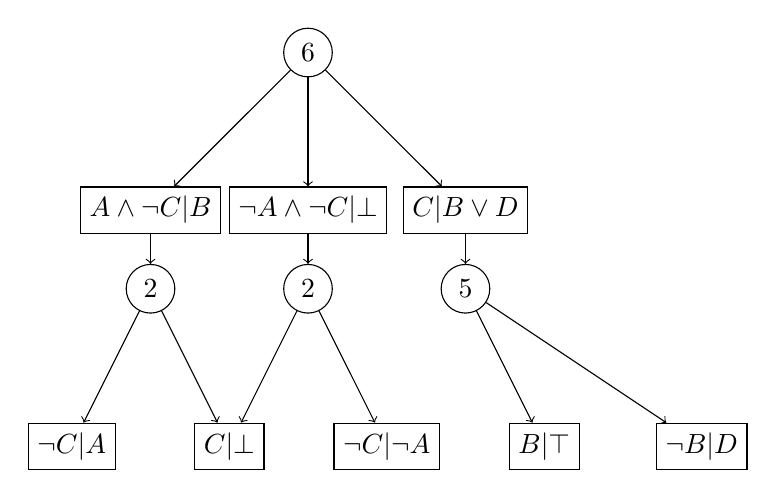
\begin{tikzpicture}[align=center]
    \node[circle,draw] at (0, 0) (x1) {6};;
    \node[rectangle,draw] at (-2, -2) (n10) {$A \land \lnot C | B$};
    \node[rectangle,draw] at (0, -2) (n11) {$\lnot A \land \lnot C | \bot$};
    \node[rectangle,draw] at (2, -2) (n12) {$C | B \lor D$};
    \node[circle,draw] at (-2, -3) (n20) {2};
    \node[circle,draw] at (0, -3) (n21) {2};
    \node[circle,draw] at (2, -3) (n22) {5};
    \node[rectangle,draw] at (-3, -5) (n30) {$\lnot C | A$};
    \node[rectangle,draw] at (-1, -5) (n31) {$C | \bot$};
    \node[rectangle,draw] at (1, -5) (n32) {$\lnot C | \lnot A$};
    \node[rectangle,draw] at (3, -5) (n33) {$B | \top$};
    \node[rectangle,draw] at (5, -5) (n34) {$\lnot B | D$};
    
    \draw[->]       (x1) -- (n10);
    \draw[->]       (x1) -- (n11);
    \draw[->]       (x1) -- (n12);
    \draw[->]       (n10) -- (n20);
    \draw[->]       (n11) -- (n21);
    \draw[->]       (n12) -- (n22);
    \draw[->]       (n20) -- (n30);
    \draw[->]       (n20) -- (n31);
    \draw[->]       (n21) -- (n31);
    \draw[->]       (n21) -- (n32);
    \draw[->]       (n22) -- (n33);
    \draw[->]       (n22) -- (n34);
\end{tikzpicture}
\end{center}

 % 5
 \clearpage
 \section{}
\renewcommand{\labelenumi}{(\alph{enumi})}
 \begin{enumerate}
\item The uncompressed partition of $f = (A \land B)\lor(B \land C)\lor(C \land D)$ for $X = \{A,B\}$ and $Y = \{C, D\}$ is:
    \begin{center}
           \begin{tabular}{ |c|c| }
            \hline
             Prime&Sub \\ 
             \hline
             $A \land B$ & $true$ \\
             \hline
             $A \land \lnot B$ & $C \land D$ \\
             \hline
             $\lnot A \land B$ & $C$ \\
             \hline
             $\lnot A \land \lnot B$ & $C \land D$ \\
             \hline
            \end{tabular} \\
    \end{center}
\item The uncompressed partition of $g = (\lnot A \land B)\lor(C \land \lnot D)$ for $X = \{A,B\}$ and $Y = \{C, D\}$ is:
    \begin{center}
           \begin{tabular}{ |c|c| }
            \hline
             Prime&Sub \\ 
             \hline
             $A \land B$ & $C \land \lnot D$ \\
             \hline
             $A \land \lnot B$ & $C \land \lnot D$ \\
             \hline
             $\lnot A \land B$ & $true$ \\
             \hline
             $\lnot A \land \lnot B$ & $C \land \lnot D$ \\
             \hline
            \end{tabular} \\
    \end{center}
\item The uncompressed partition of $f \lor g$ for $X = \{A,B\}$ and $Y = \{C, D\}$ is:
    \begin{center}
           \begin{tabular}{ |c|c| }
            \hline
             Prime&Sub \\ 
             \hline
             $A \land B$ & $true$ \\
             \hline
             $A \land \lnot B$ & $C$ \\
             \hline
             $\lnot A \land B$ & $true$ \\
             \hline
             $\lnot A \land \lnot B$ & $C$ \\
             \hline
            \end{tabular} \\
    \end{center}
    Which compresses to:
    \begin{center}
           \begin{tabular}{ |c|c| }
            \hline
             Prime&Sub \\ 
             \hline
             $B$ & $true$ \\
             \hline
             $\lnot B$ & $C$ \\
             \hline
            \end{tabular} \\
    \end{center}
    This equivalent to $h = (B \lor C)$.
\end{enumerate}
 % 6
 \clearpage
 \section{}
 \[(\lnot A \lor B \lor \lnot C) \land (\lnot A \lor B \lor C) \land (A \lor \lnot B \lor \lnot C) \land (A \lor \lnot B \lor C) \land (A \lor B \lor C)\]
 The prime implicates produced by resolution of original terms:
 \[
    (\lnot A \lor B) \land (A \lor \lnot B) \land (A \lor C) \land (B \lor C)
\]
 % 7
 \clearpage
 \section{}
 \renewcommand{\labelenumi}{}
 \begin{enumerate}
\item MC:\\
 The largest set of features that can be turned off (to 0) from the world $(S=1, G=1, F=1, M=0)$ is 2 and the two worlds which satisfy that are $(S=0, G=0, F=1, M=0)$ and $(S=0, G=1, F=0, M=0)$.
\item PI:\\
The smallest feature set $\alpha$ of the instance $(S=1, G=0, F=1, M=1)$ which creates a remaining arbitrary feature set $\beta$ is: \\
$\alpha = \{F=1, M=1\}$ \\
$\beta = \{S=1/0, G=1/0\}$
\end{enumerate}
 

% 8
\clearpage
\section{}
\[ \Delta = \begin{cases} 
      ok_1 \Rightarrow (A \Leftrightarrow \lnot B)\\
      ok_2 \Rightarrow (A \land B) \Leftrightarrow C\\
   \end{cases}
\]
\renewcommand{\labelenumi}{}
\begin{enumerate}
\item The kernel and MC diagnosis when the output is true:
\[Health(\Delta, C) = \lnot ok_1 \lor \lnot ok_2\]
\begin{center}
           \begin{tabular}{ |c|c|c| }
            \hline
             $ok_1$&$ok_2$&Diagnosis for C? \\ 
             \hline
             \checkmark & \checkmark & no \\
             \hline
             \checkmark & $\times$ & yes \\
             \hline
             $\times$ & \checkmark & yes \\
             \hline
             $\times$ & $\times$ & yes \\
             \hline
            \end{tabular} \\
    \end{center}
    The minimum cardinality is 1 in this case.
\item The kernel and MC diagnosis when the output is false:
    \[Health(\Delta, \lnot C) = true\]
    \begin{center}
               \begin{tabular}{ |c|c|c| }
                \hline
                 $ok_1$&$ok_2$&Diagnosis for $\lnot C$? \\ 
                 \hline
                 \checkmark & \checkmark & yes \\
                 \hline
                 \checkmark & $\times$ & yes \\
                 \hline
                 $\times$ & \checkmark & yes \\
                 \hline
                 $\times$ & $\times$ & yes \\
                 \hline
                \end{tabular} \\
        \end{center}
        The minimum cardinality is 0.
\end{enumerate}
\end{document}